\begin{center}
    \captionof{figure}{Within- and Between-Person Effects of Binary Predictor and Continuous Outcome}

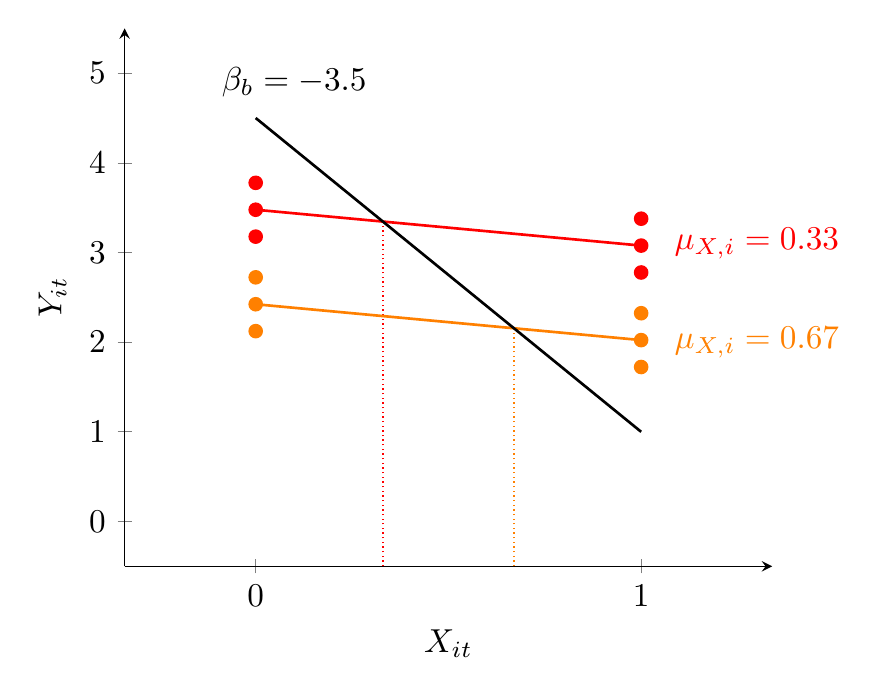
\begin{tikzpicture}[scale=1.2]
    \begin{axis}[
        axis x line=left, 
        axis y line=left, 
        xlabel={$X_{it}$}, ylabel={$Y_{it}$},
        xmin=-0.2, xmax=1.2, ymin=0, ymax=5,
        xtick={0,1},
        ytick={0,1,2,3,4,5},
        enlargelimits=true,
        clip=false,
        xshift=-15mm
    ]

    \pgfmathsetmacro{\gammaZero}{4.5}
    \pgfmathsetmacro{\gammaOne}{-3.1}
    \pgfmathsetmacro{\betaOne}{-0.4}
    \pgfmathsetmacro{\betaB}{-3.5}

    % === Person with mu_X = 0.33 ===
    \pgfmathsetmacro{\muXone}{0.33}
    \pgfmathsetmacro{\intOne}{\gammaZero + \gammaOne*\muXone}
    \addplot[thick, red] coordinates {
        (0, {\intOne + \betaOne*0})
        (1, {\intOne + \betaOne*1})
    };
    \addplot[only marks, red] coordinates {
        (0, {\intOne + \betaOne*0})
        (0, {\intOne + \betaOne*0.75})
        (0, {\intOne + \betaOne*-0.75})
        (1, {\intOne + \betaOne*0.25})
        (1, {\intOne + \betaOne*1})
        (1, {\intOne + \betaOne*1.75})
    };
    \addplot[densely dotted, thin, red] coordinates {
        (\muXone, -0.5)
        (\muXone, {\gammaZero + \betaB*\muXone})
    };

    % === Person with mu_X = 0.67 ===
    \pgfmathsetmacro{\muXtwo}{0.67}
    \pgfmathsetmacro{\intTwo}{\gammaZero + \gammaOne*\muXtwo}
    \addplot[thick, orange] coordinates {
        (0, {\intTwo + \betaOne*0})
        (1, {\intTwo + \betaOne*1})
    };
    \addplot[only marks, orange] coordinates {
        (0, {\intTwo + \betaOne*0})
        (0, {\intTwo + \betaOne*0.75})
        (0, {\intTwo + \betaOne*-0.75})
        (1, {\intTwo + \betaOne*0.25})
        (1, {\intTwo + \betaOne*1})
        (1, {\intTwo + \betaOne*1.75})
    };
    \addplot[densely dotted, thin, orange] coordinates {
        (\muXtwo, -0.5)
        (\muXtwo, {\gammaZero + \betaB*\muXtwo})
    };

    % === Between-person regression line ===
    \addplot[thick, black, domain=0:1] {\gammaZero + \betaB*x};

    % === Labels ===
    \node[red] at (axis cs:1.3,3.1) {$\mu_{X,i}=0.33$};
    \node[orange] at (axis cs:1.3,2.0) {$\mu_{X,i}=0.67$};
    \node[black] at (axis cs:0.1,4.9) {$\beta_\text{b} = -3.5$};

    \end{axis}
\end{tikzpicture}

    \label{fig:withinbetween-binxconty}
    \begin{figurenote}
        The solid black slope represents the between-person effect and the colored slopes the within-cluster effects. The X-axis simultaneously represents $X_{it}$ for the within-slope and $\mu_{X,i}$ for the between-slope; and the Y-axis represents $Y_{it}$ for the within slope and $Y_i$ for the between-slope. Dots reflect possible datapoints and diamonds reflect the position of $\mu_{X,i}$ on the within-person slope.
    \end{figurenote}
\end{center}